\documentclass[serif]{beamer}\usepackage[]{graphicx}\usepackage[]{color}
%% maxwidth is the original width if it is less than linewidth
%% otherwise use linewidth (to make sure the graphics do not exceed the margin)
\makeatletter
\def\maxwidth{ %
  \ifdim\Gin@nat@width>\linewidth
    \linewidth
  \else
    \Gin@nat@width
  \fi
}
\makeatother

\definecolor{fgcolor}{rgb}{0.345, 0.345, 0.345}
\newcommand{\hlnum}[1]{\textcolor[rgb]{0.686,0.059,0.569}{#1}}%
\newcommand{\hlstr}[1]{\textcolor[rgb]{0.192,0.494,0.8}{#1}}%
\newcommand{\hlcom}[1]{\textcolor[rgb]{0.678,0.584,0.686}{\textit{#1}}}%
\newcommand{\hlopt}[1]{\textcolor[rgb]{0,0,0}{#1}}%
\newcommand{\hlstd}[1]{\textcolor[rgb]{0.345,0.345,0.345}{#1}}%
\newcommand{\hlkwa}[1]{\textcolor[rgb]{0.161,0.373,0.58}{\textbf{#1}}}%
\newcommand{\hlkwb}[1]{\textcolor[rgb]{0.69,0.353,0.396}{#1}}%
\newcommand{\hlkwc}[1]{\textcolor[rgb]{0.333,0.667,0.333}{#1}}%
\newcommand{\hlkwd}[1]{\textcolor[rgb]{0.737,0.353,0.396}{\textbf{#1}}}%
\let\hlipl\hlkwb

\usepackage{framed}
\makeatletter
\newenvironment{kframe}{%
 \def\at@end@of@kframe{}%
 \ifinner\ifhmode%
  \def\at@end@of@kframe{\end{minipage}}%
  \begin{minipage}{\columnwidth}%
 \fi\fi%
 \def\FrameCommand##1{\hskip\@totalleftmargin \hskip-\fboxsep
 \colorbox{shadecolor}{##1}\hskip-\fboxsep
     % There is no \\@totalrightmargin, so:
     \hskip-\linewidth \hskip-\@totalleftmargin \hskip\columnwidth}%
 \MakeFramed {\advance\hsize-\width
   \@totalleftmargin\z@ \linewidth\hsize
   \@setminipage}}%
 {\par\unskip\endMakeFramed%
 \at@end@of@kframe}
\makeatother

\definecolor{shadecolor}{rgb}{.97, .97, .97}
\definecolor{messagecolor}{rgb}{0, 0, 0}
\definecolor{warningcolor}{rgb}{1, 0, 1}
\definecolor{errorcolor}{rgb}{1, 0, 0}
\newenvironment{knitrout}{}{} % an empty environment to be redefined in TeX

\usepackage{alltt}
\usetheme{Boadilla}
\usepackage{graphicx}
\usepackage{xcolor}
\usepackage{booktabs}
\usepackage{tikz}
\usetikzlibrary{decorations.pathreplacing}
\usetikzlibrary{shapes,arrows,positioning,shadows}
\usepackage{pgf}
\usepackage{caption}
\usepackage[absolute,overlay]{textpos}
% \usepackage[texcoord, grid,gridcolor=red!10,subgridcolor=green!10,gridunit=pt]{eso-pic}

% change format of enumerated lists
\setbeamertemplate{enumerate items}[default]
\setbeamertemplate{navigation symbols}{}

% macros
\newcommand{\emtxt}[1]{\textbf{\textit{{\color{mypal4} #1}}}}
\definecolor{mycol1}{rgb}{0.65,0.8,0.89}
\definecolor{mycol2}{rgb}{0.98,0.6,0.6}

% change font size for figure captions
\setbeamerfont{caption}{size=\scriptsize}

\newcommand\FrameText[1]{%
  \begin{textblock*}{\paperwidth}(20pt,50pt)
    \raggedright #1\hspace{.5em}
  \end{textblock*}}

% custom colors
\definecolor{mypal1}{HTML}{F0F9E8}\definecolor{mypal2}{HTML}{BAE4BC}\definecolor{mypal3}{HTML}{7BCCC4}\definecolor{mypal4}{HTML}{43A2CA}\definecolor{mypal5}{HTML}{0868AC}

% knitr setup


% dependent data


% get online bib file



\setbeamercolor{title}{fg=mypal5} % main title
\setbeamercolor{frametitle}{fg=mypal4, bg=mypal2} % frame titles
\setbeamercolor{structure}{fg=mypal4} % bottom banner
\setbeamercolor{normal text}{fg=mypal5}
\usebackgroundtemplate{
\includegraphics[height=\paperheight,width=\paperwidth]{fig/back_tmp.pdf}}
\IfFileExists{upquote.sty}{\usepackage{upquote}}{}
\begin{document}

\title[Risk assessment for CA lakes]{\textbf{Landscape scale risk assessment of cyanobacteria blooms in California lakes}}
\author[Beck et al.]{Marcus W. Beck$^1$, Martha Sutula, Meredith Howard, Eric Stein}

\institute[SCCWRP]{$^1$Southern California Coastal Water Research Project, Costa Mesa, CA \href{mailto:marcusb@sccwrp.org}{marcusb@sccwrp.org}, Phone: 714-755-3217}

\date{May 24\textsuperscript{th}, 2018}

\titlegraphic{
\centerline{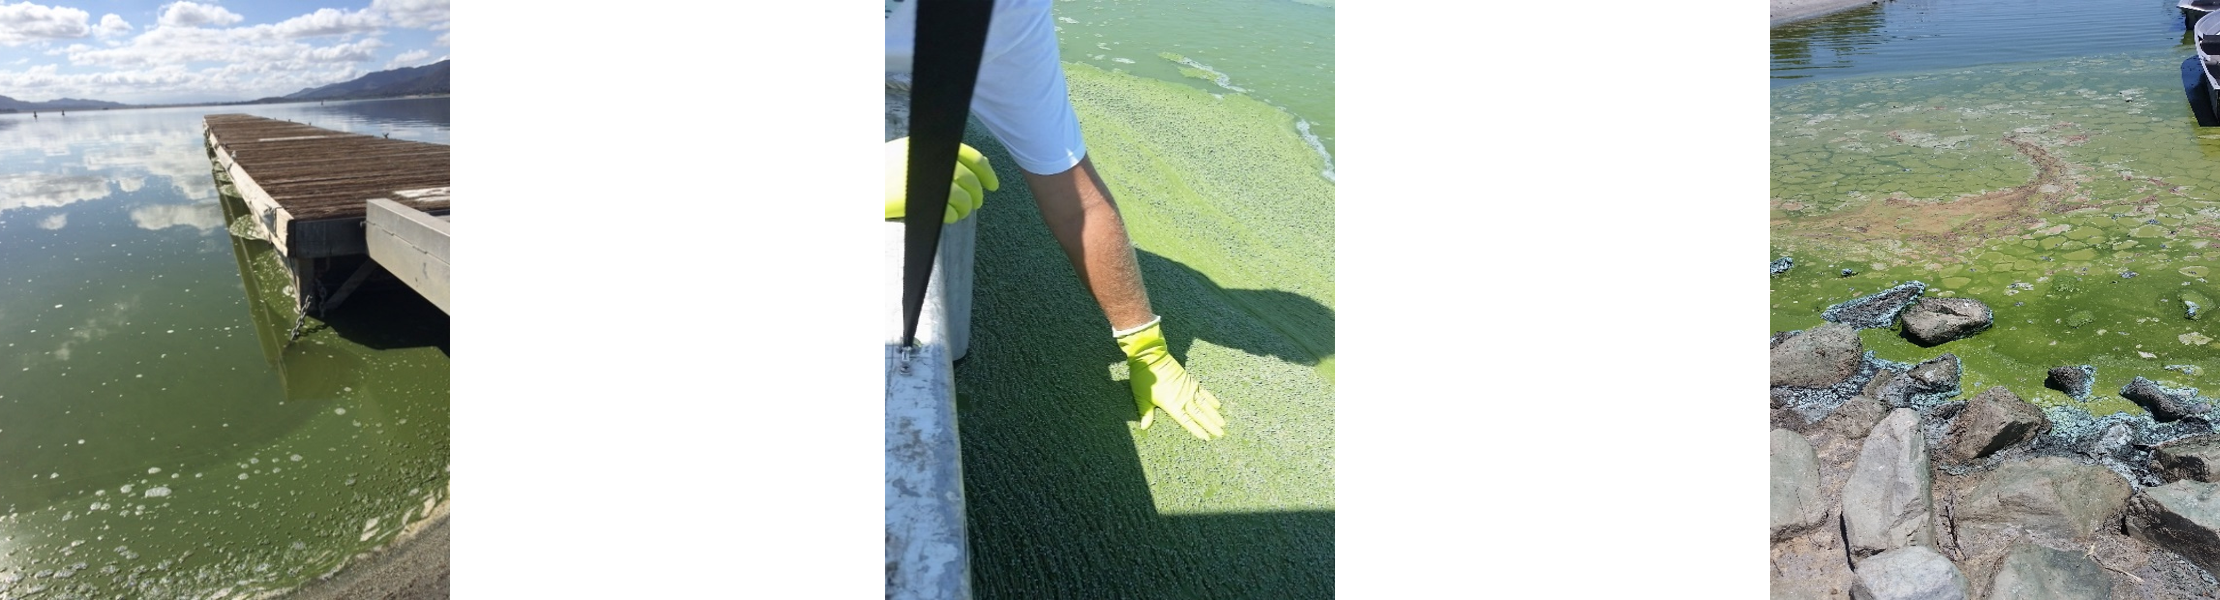
\includegraphics[width=0.8\linewidth]{fig/elsinore.png}}
\vspace{0.1in}
}

%%%%%%
\begin{frame}[shrink]
\vspace{0.2in}
\titlepage
\end{frame}

\section{Background}

%%%%%%
\begin{frame}{{$\vcenter{\hbox{
\includegraphics[width=0.07\paperwidth]{fig/sccwrp_logo.png}}}$\hspace{0.07in}\textbf{California lakes have a HAB problem}}}
\begin{columns}
\begin{column}{0.4\textwidth}
\begin{itemize}
\item 2017 targeted sampling on Labor Day revealed a problem \\~\\
\item Over half of sampled lakes exceeded a proposed recreational criteria
\end{itemize}
\end{column}
\begin{column}{0.6\textwidth}
\centerline{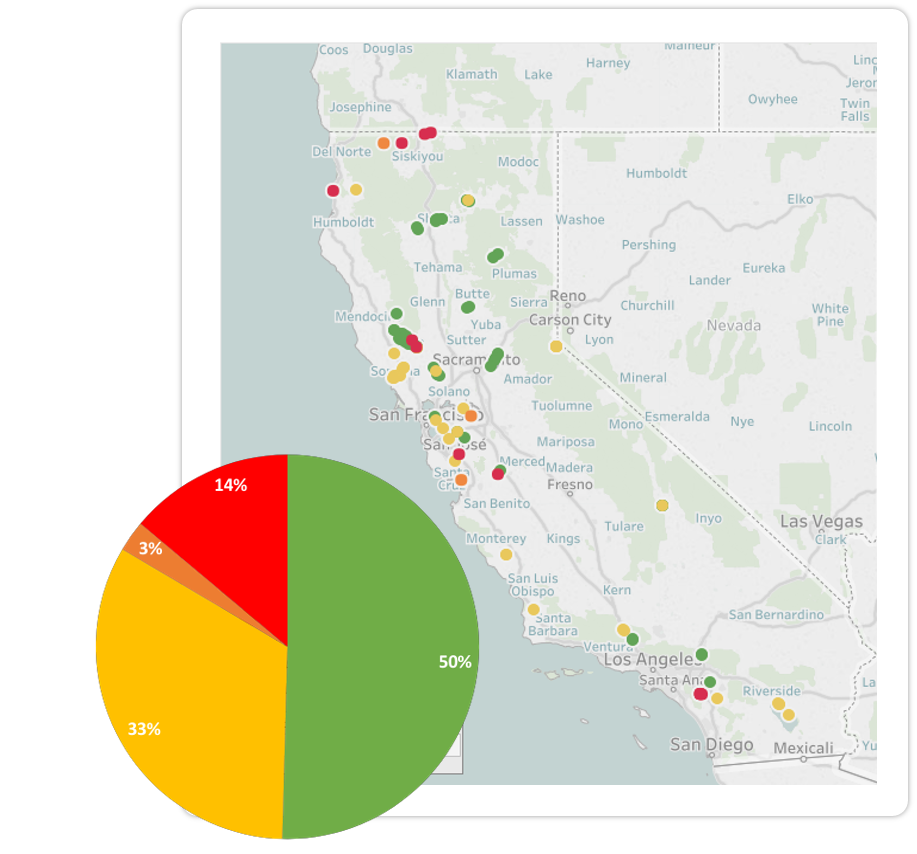
\includegraphics[width=\textwidth]{fig/swamp_holiday2.png}}
\end{column}
\end{columns}
\end{frame}

%%%%%%
\begin{frame}[t]{{$\vcenter{\hbox{
\includegraphics[width=0.07\paperwidth]{fig/sccwrp_logo.png}}}$\hspace{0.07in}\textbf{California lakes have a data problem}}}
Limited \textit{in situ} data for California, tons of watershed data
\vspace{-0.15in}
\begin{columns}[t]
\begin{column}{0.5\textwidth}


{\centering 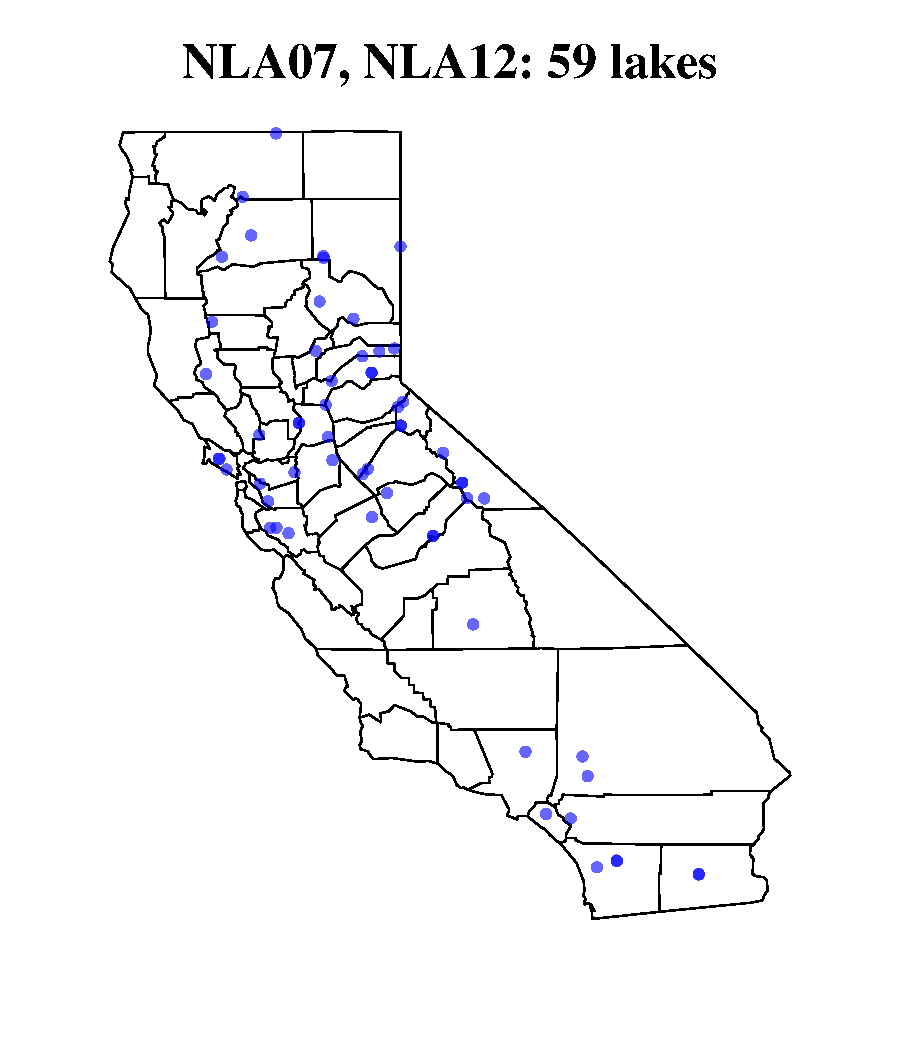
\includegraphics[width=\maxwidth]{fig/unnamed-chunk-2-1} 

}



\end{column}
\begin{column}{0.5\textwidth}


{\centering 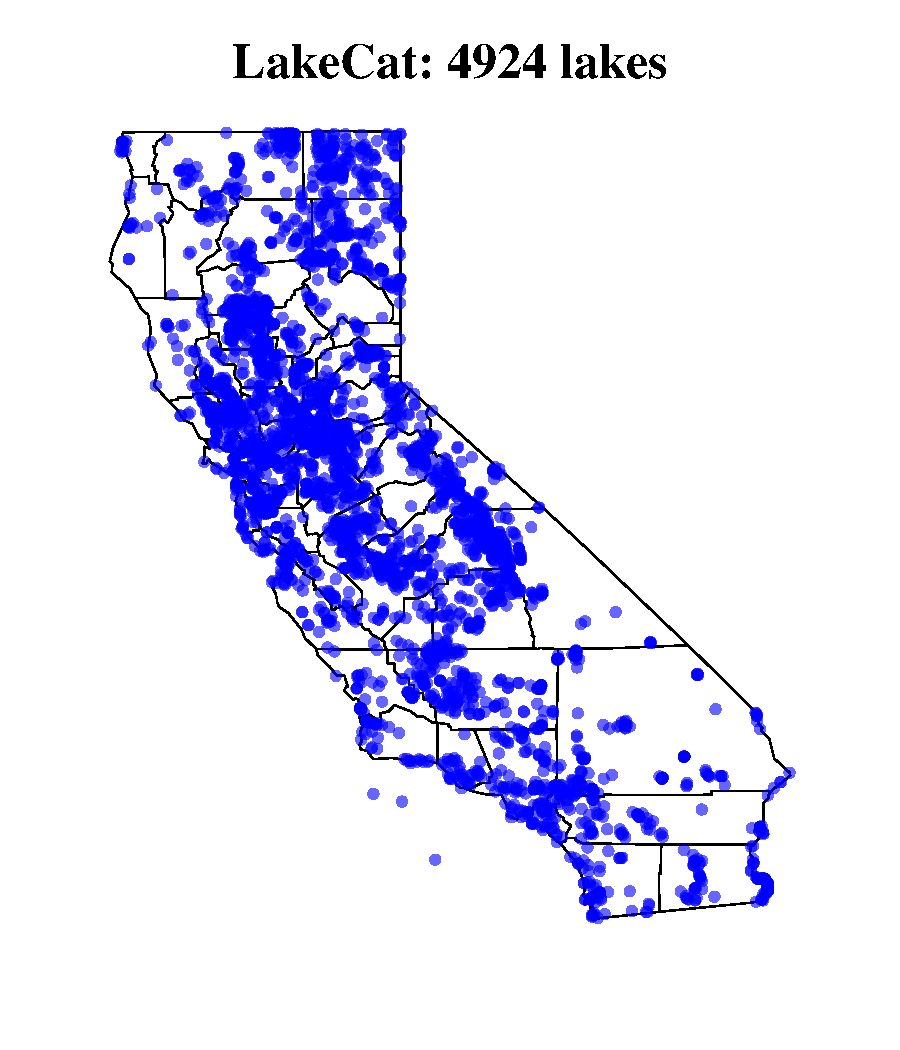
\includegraphics[width=\maxwidth]{fig/unnamed-chunk-3-1} 

}



\end{column}
\end{columns}
\vspace{-0.15in}
{\tiny
\cite{USEPA09,USEPA17,Hill18}
}
\end{frame}

%%%%%%
\begin{frame}{{$\vcenter{\hbox{
\includegraphics[width=0.07\paperwidth]{fig/sccwrp_logo.png}}}$\hspace{0.07in}\textbf{Develop a screening tool for HAB risk}}}
\onslide<1->
Despite the problem, we have no formal bioassessment methods for lakes \\~\\
\begin{itemize}
\item<+-> Current thresholds and reporting are voluntary
\item<+-> No recommendations for regional water boards on listing/delisting or where to monitor
\item<+-> Data limitations make it difficult to identify spatial/temporal trends\\~\\
\end{itemize}
\onslide<+->
\begin{center}
\emtxt{Goal: develop screening tool to evaluate the relative risk of lakes exceeding a eutrophication endpoint related to bloom occurrence}
\end{center}
\end{frame}

%%%%%%
\begin{frame}{{$\vcenter{\hbox{
\includegraphics[width=0.07\paperwidth]{fig/sccwrp_logo.png}}}$\hspace{0.07in}\textbf{Develop a screening tool for HAB risk}}}
\onslide<1->
A four-step approach to identify risk from a limited dataset:\\~\\
\begin{enumerate}
\item<+-> Develop link between chlorophyll and microcystin
\item<+-> Develop link between chlorophyll and location using spatial model
\item<+-> Predict statewide risk from chlorophyll prediction from landscape position
\item<+-> Identify landscape factors that are related to risk \\~\\
\end{enumerate}
\onslide<+->
\begin{center}
\emtxt{An exercise in diminishing returns...}
\end{center}
\end{frame}

%%%%%%
\begin{frame}{{$\vcenter{\hbox{
\includegraphics[width=0.07\paperwidth]{fig/sccwrp_logo.png}}}$\hspace{0.07in}\textbf{Modelling approach}}}
\begin{overprint}
\only<2>{
\FrameText{\huge{\textbf{1}}}
}
\only<3>{
\FrameText{\huge{\textbf{2}}}
}
\only<4>{
\FrameText{\huge{\textbf{3}}}
}
\only<5>{
\FrameText{\huge{\textbf{4}}}
}
\centering
\includegraphics<1>[width = 0.95\textwidth]{fig/schem.png}
\includegraphics<2>[width = 0.95\textwidth]{fig/schem1.png}
\includegraphics<3>[width = 0.95\textwidth]{fig/schem2.png}
\includegraphics<4>[width = 0.95\textwidth]{fig/schem3.png}
\includegraphics<5>[width = 0.95\textwidth]{fig/schem4.png}
\end{overprint}
\end{frame}



%%%%%%
\begin{frame}{{$\vcenter{\hbox{
\includegraphics[width=0.07\paperwidth]{fig/sccwrp_logo.png}}}$\hspace{0.07in}\textbf{1) Link between chlorophyll and microcystin}}}
\begin{columns}
\begin{column}{0.6\textwidth}
\begin{center}
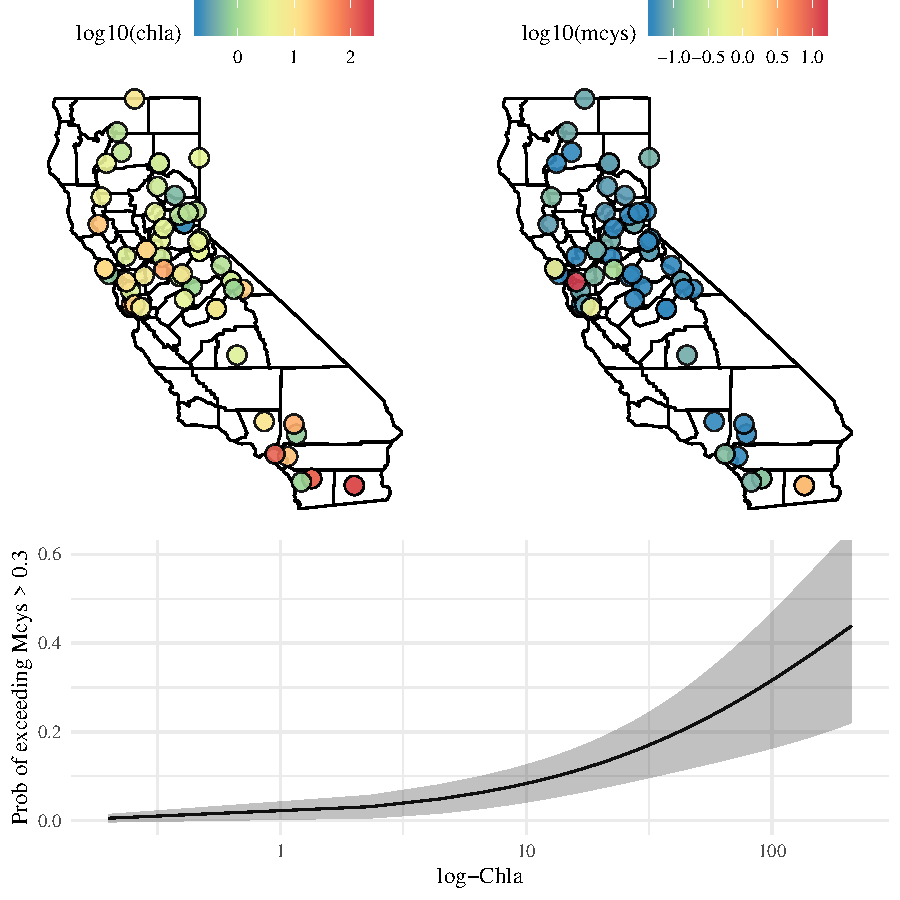
\includegraphics[width = \textwidth]{fig/modmcy.pdf}
\end{center}
\end{column}
\begin{column}{0.4\textwidth}
\begin{itemize}
\item \textit{In situ} NLA data as probabilistic survey\\~\\
\item Build a simple model of the likelihood of exceeding some threshold \\~\\
\item Define a criteria threshold, arbitrary at this point
\end{itemize}
\end{column}
\end{columns}
\end{frame}





%%%%%%
\begin{frame}{{$\vcenter{\hbox{
\includegraphics[width=0.07\paperwidth]{fig/sccwrp_logo.png}}}$\hspace{0.07in}\textbf{2) Link between chlorophyll and location}}}
\centering
\emtxt{Using a spatial model to predict chlorophyll from location} \\~\\
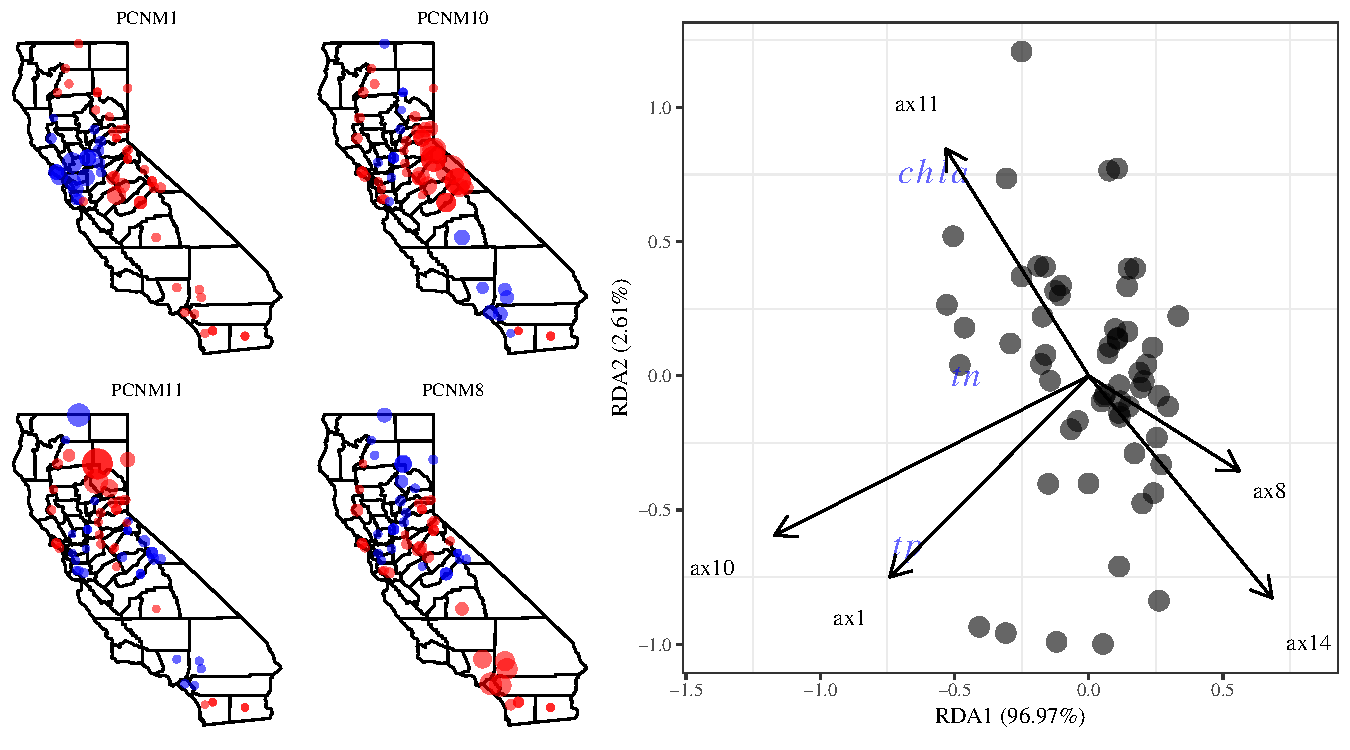
\includegraphics[width = \textwidth]{fig/pcnm.pdf}
\end{frame}



%%%%%%
\begin{frame}{{$\vcenter{\hbox{
\includegraphics[width=0.07\paperwidth]{fig/sccwrp_logo.png}}}$\hspace{0.07in}\textbf{2) Link between chlorophyll and location}}}
\centering
\emtxt{Predicted chlorophyll from location seems okay} \\~\\
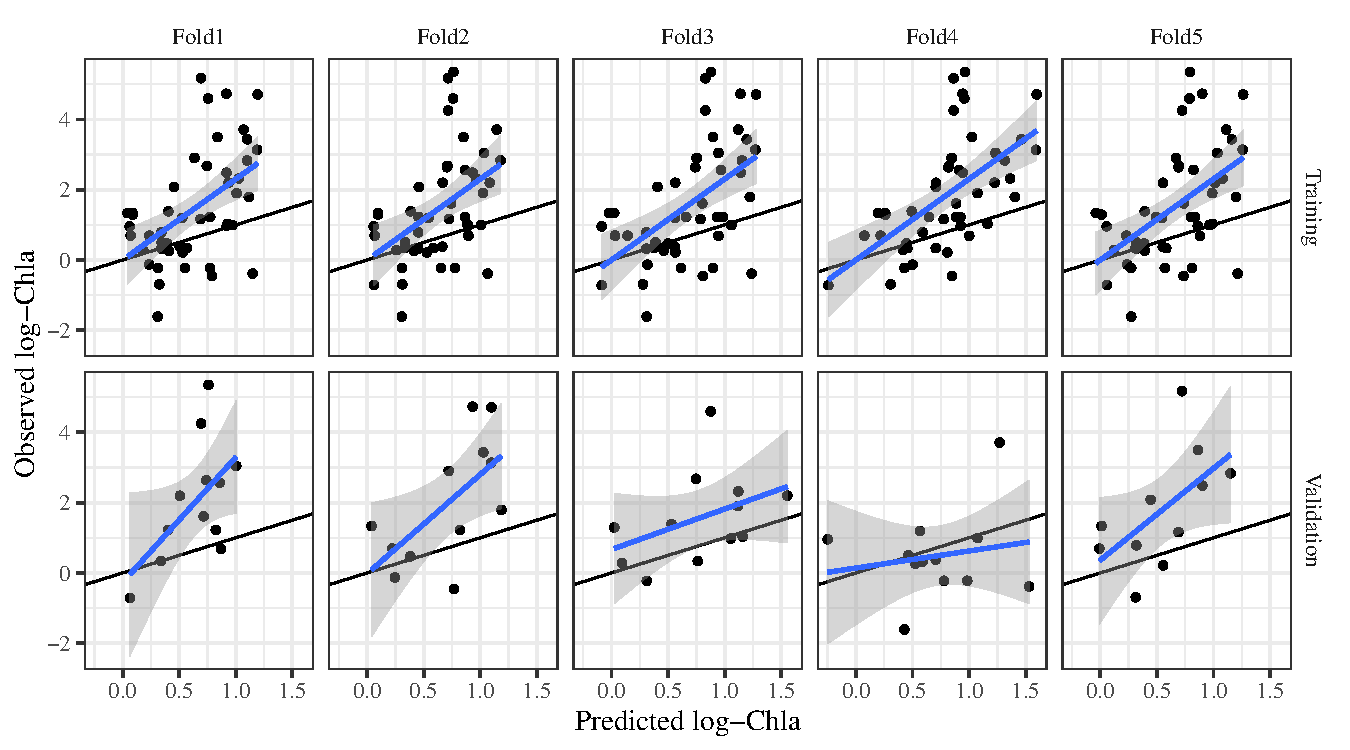
\includegraphics[width = \textwidth]{fig/modval.pdf}
\end{frame}



%%%%%%
\begin{frame}{{$\vcenter{\hbox{
\includegraphics[width=0.07\paperwidth]{fig/sccwrp_logo.png}}}$\hspace{0.07in}\textbf{3) Estimated risk from chla prediction}}}
\emtxt{An additional leap: Use predicted chlorophyll from landscape model, estimate predicted probability of exceeding threshold, categorize relative risk} \\~\\
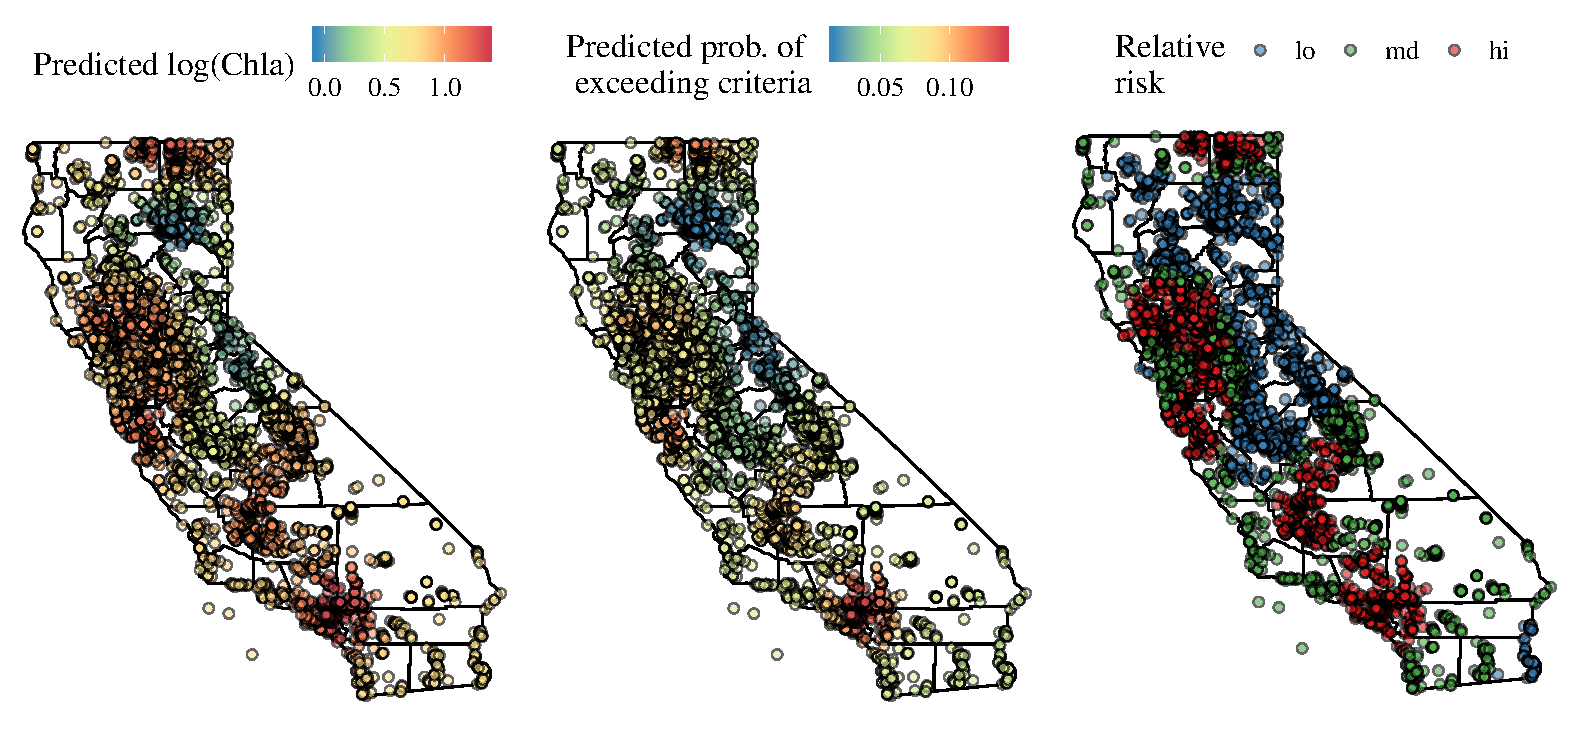
\includegraphics[width = \textwidth]{fig/rskprd.pdf}
\end{frame}



%%%%%%
\begin{frame}{{$\vcenter{\hbox{
\includegraphics[width=0.07\paperwidth]{fig/sccwrp_logo.png}}}$\hspace{0.07in}\textbf{4) Identify landscape factors related to risk}}}
\emtxt{Top five most important watershed factors linked to risk categories} \\~\\
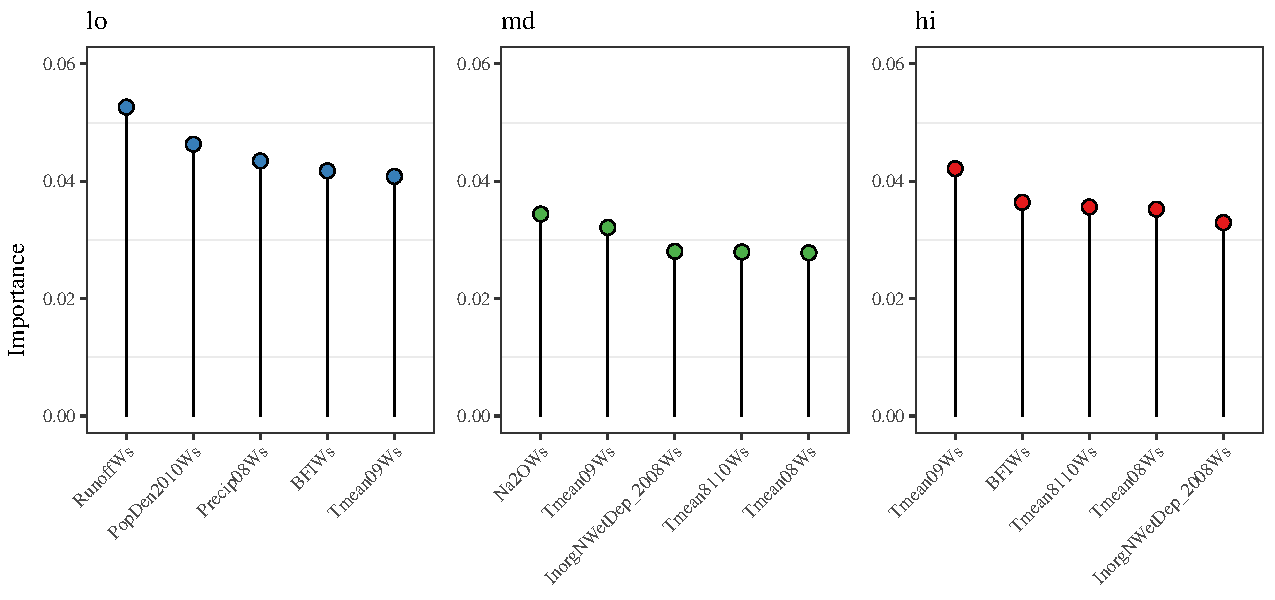
\includegraphics[width = \textwidth]{fig/rskfac.pdf}
\end{frame}

%%%%%%
\begin{frame}{{$\vcenter{\hbox{
\includegraphics[width=0.07\paperwidth]{fig/sccwrp_logo.png}}}$\hspace{0.07in}\textbf{A vision for lake bioassessment in CA}}}
\begin{itemize}
\item<+-> Despite limited data, we effectively screened lakes by HAB risk \\~\\
\item<+-> Relatively low risk in the Sierra Nevada, North Coasts, portions of Central Valley\\~\\
\item<+-> Higher risk in Chapparal, Desert, Urban centers \\~\\
\item<+-> Landscape position is a potentially powerful predictor of water quality \\~\\
\end{itemize}
\onslide<1->
\centerline{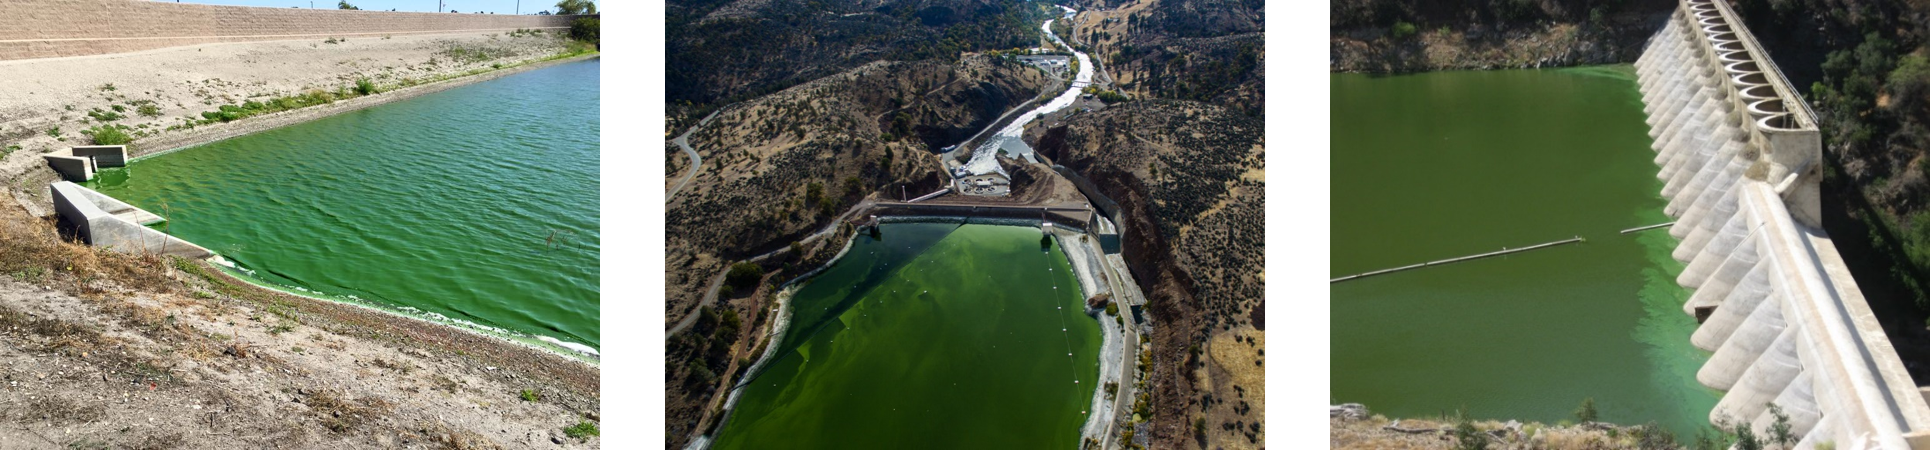
\includegraphics[width=0.8\textwidth]{fig/habex.png}}
\end{frame}



%%%%%%
\begin{frame}{{$\vcenter{\hbox{
\includegraphics[width=0.07\paperwidth]{fig/sccwrp_logo.png}}}$\hspace{0.07in}\textbf{A vision for lake bioassessment in CA}}}
\begin{columns}
\begin{column}{0.5\textwidth}
\begin{itemize}
\item Alternative data acquisition can be explored to further assess risk \\~\\
\item Additional \textit{in situ} and probabilistic sampling needed \\~\\
\item Leverage both for rapid response to bloom incidence
\end{itemize}
\end{column}
\begin{column}{0.5\textwidth}
\centerline{
\includegraphics[width=0.7\textwidth]{fig/cyan.png}}\\~\\
\centerline{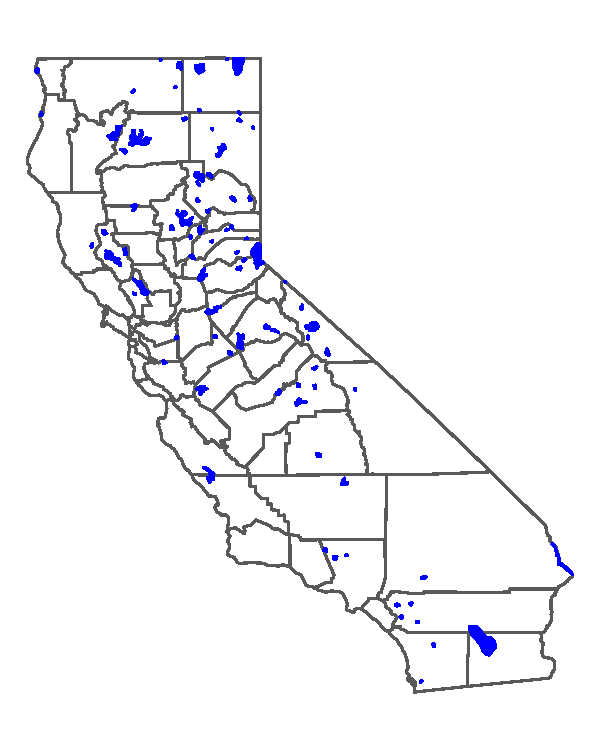
\includegraphics[width=0.5\textwidth]{fig/cyanca.pdf}}
\end{column}
\end{columns}
\vspace{0.1in}
\centerline{{\tiny \url{https://www.epa.gov/water-research/cyanobacteria-assessment-network-cyan}}}
\end{frame}

%%%%%%
\begin{frame}
\emtxt{Acknowledgments}:\\~\\
\begin{columns}
\begin{column}{0.8\textwidth}
{\footnotesize
Research staff and employees at Southern California Coastal Water Research Project\\~\\
Blake Schaeffer (USEPA, ORD) for CyAN data\\~\\
Ryan Hill (USEPA, ORISE) for LakeCat data\\~\\
Photo credits: Meredith Howard, Susan Fricke, Carey Nagoda \\~\\}
\end{column}
\begin{column}{0.2\textwidth}
\end{column}
\end{columns}
\vfill
\emtxt{Funding sources and contact}:\\~\\
\begin{columns}
\begin{column}{0.5\textwidth}
\vfill
\centerline{
\includegraphics[width=0.6\linewidth]{fig/sccwrp_logo.png}}
\vfill
\end{column}
\begin{column}{0.5\textwidth}
\scriptsize
\href{mailto:marcusb@sccwrp.org}{marcusb@sccwrp.org}, 7147553217\\~\\

\includegraphics[width = 0.05\textwidth]{fig/git.png} GitHub (project): \href{https://github.com/fawda123/cali_lake}{https://github.com/fawda123/cali\_lake}\\~\\

\includegraphics[width = 0.05\textwidth]{fig/git.png} GitHub (presentation): \href{https://github.com/fawda123/SFS_2018}{https://github.com/fawda123/SFS\_2018}\\~\\

\includegraphics[width = 0.05\textwidth]{fig/twitter.png} Twitter: @fawda123
\end{column}
\end{columns}
\vspace{0.2in}
\end{frame}

%%%%%%
\section{References}
\begin{frame}[t,shrink]{\textbf{References}}
\tiny
\setbeamertemplate{bibliography item}{}
\bibliographystyle{apalike_mine}
% \bibliography{refs}
\bibliography{refsnew}
\end{frame}

\end{document}
